\documentclass[xetex, handout]{beamer}
\usetheme{hsr}

\usepackage[T1]{fontenc}
\usepackage{cmbright}
\usepackage{unicode-math}

\usefonttheme{structurebold}

\usepackage{amsmath}
\usepackage{amssymb}

\usepackage{tikz}
\usetikzlibrary{trees}

\usetikzlibrary{backgrounds}
\usetikzlibrary{bending}
\usetikzlibrary{calc}
\usetikzlibrary{decorations.pathreplacing}
\usetikzlibrary{fadings}
\usetikzlibrary{matrix}
\usetikzlibrary{positioning}

\pgfdeclarelayer{bg}
\pgfsetlayers{bg,main}

\tikzset{
  db/.pic={
    \draw[white, fill=white](-.6,0) rectangle (.6,1.4);
    \draw[white, fill=white](0,1.4) ellipse [x radius=.6,y radius=.15];
    \foreach \y in {0,.5,1}
    {
      \draw[thick, fill=white]
        (-0.6,\y) to [looseness=0.5,bend right=90] ++(1.2,0)
              to ++(0,0.4)
              to [looseness=0.5,bend left=90] ++(-1.2,0)
              to ++(0,-0.4);
      \draw[thick] (-0.6,\y+0.4) edge[looseness=0.5,bend left=90] ++(1.2,0);
    }
  },
  pics/file/.style args = {#1 #2 #3}{
    code = {
      % Rectangle
      \node[
        outer sep = 0, inner sep = 0,
        minimum width = 1cm, minimum height = 1.2cm,
        #3
      ] (#1) {#2};
      % Paper outline
      \draw[thick, fill = white]
        ({#1}.north west) -- ($({#1}.north east) - (.3,0)$)
          -- ++(0,-.3) -- ++(.3,0) -- ({#1}.south east)
          -- ({#1}.south west) -- ({#1}.north west) -- cycle;
      % Fill inside paper
      \draw[fill = white] 
        ($({#1}.north east) - (.3,0)$) to ++(0,-.3) 
        to ++(.3,0) to ++(-.3,.3) to cycle;
      % Paper angle
      \draw[black, thick] ($({#1}.north east) - (.3,0)$) to ++(.3,-.3);
      % Text inside paper
      \node[
        outer sep = 1mm,
        inner sep = 0,
        minimum width = 1cm,
        minimum height = 1.2cm,
      ] (#1) at (#1) {#2};
    },
  },
}


\title{Introduction to Git}
\author{
  Naoki Pross --- \texttt{np@0hm.ch}
}
\institute{}

\date{XX. March 2025}

\AtBeginSection[]
{
  \begin{frame}[shrink]{Table of Contents}
    \tableofcontents[
      currentsection,
      hideothersubsections,
      sectionstyle=show/shaded,
    ]
  \end{frame}
}

\begin{document}

\frame{\titlepage}

\section{The Problem}

\begin{frame}{What do we want?}
  \begin{alertblock}{The Problem}
    Synchronize data across multiple computers, with multiple people working on
    (possibly the same) files.
  \end{alertblock}
  \pause

  \begin{block}{Linus' Wishes (The guy who invented Git)}
    \begin{itemize}
      \item Synchronization \emph{always} works
      \item Teamwork is possible and efficient
      \item Works offline
      \item Fast
    \end{itemize}
    \emph{intuitive or easy to use} was not on his list!
  \end{block}
\end{frame}

\begin{frame}{Other Solutions?}
  \begin{block}{Other Tools at Linus' Time}
    \begin{description}
      \item[CVS] Slow to synchronize. CVS requires a centralized server which
        can get overloaded, was usually set up by the company IT.
      \item[E-Mail] People sent patch files to each other via email.
    \end{description}
  \end{block}
  \begin{block}{Other Tools Today}
    \begin{description}
      \item[Cloud Storage] Does not work offline. Their whole business model is
        against you. You have no (real) control over when to sync.

      \item[Mercurial (hg)] Learn to walk (Git) before you run.
    \end{description}
  \end{block}
\end{frame}

\section{The Solution}

\begin{frame}{Solving the Problem: Snapshots}
  \begin{center}
    \begin{tikzpicture}
    \node at (-1, 2) [draw, fill=gray!15, thick, font=\ttfamily, left] (P) {Project/};
    \pause
    \draw[black, thick, ->] (P.north east) ++(.2,-.2) arc (-90:180:.5)
        node[pos=.6, above]{Changes};
    \draw[black, thick, ->] (0, 0) -- (7.2, 0) node [below] {Time};
    \foreach \x/\t in {0/16:04:28, 2/16:37:01, 4/17:15:44, 6/18:01:03}
    {
        \pause
        \draw[color=black, fill=magenta, thick] (\x, 0) circle (.12)
            node[below=5pt, anchor=east, rotate=70, font=\ttfamily, align=right] {\tiny 2019-09-18\\\small\t};
        \draw[thick, ->, gray] (-.8, 2) to[bend left, in=120] (\x, .2);
    }
    \end{tikzpicture}
  \end{center}
\end{frame}

\subsection{Concurrent Changes: Commit Graph}

\begin{frame}[fragile]{Solving the Problem: Concurrent Changes I}
  \begin{tikzpicture}[
      commit/.style = {
        draw, fill=orange, circle, thick,
        minimum size = 2.5mm, inner sep = 0, outer sep = 1mm,
      },
    ]
    \matrix (m) [
      column sep = 18mm, row sep = 1cm,
      row 2/.style = {row sep = 5mm},
    ] {
        \pic{file = {fb0 f {}}}; 
      & \pic{file = {fb1 f {}}}; 
      & \pic{file = {fb2 f {}}}; 
      & \pic{file = {fb3 f {}}}; 
      \\
        \node[commit, label={60:A}] (cb0) {};
      & \node[commit, label={60:B}] (cb1) {};
      & \node[commit, label={60:C}] (cb2) {};
      & \node[commit, label={60:M}, fill=magenta] (cb3) {};
        \fill[opacity=.2, magenta] (cb3) circle (5mm);
      \\
      & \node[commit, label={60:B'}] (ca1) {};
      & \node[commit, label={60:C'}] (ca2) {};
      \\
        \pic{file = {fa0 f {}}}; 
      & \pic{file = {fa1 f {}}}; 
      & \pic{file = {fa2 f {}}}; 
      & \pic{file = {fa3 f {}}}; 
      \\
    };

    \node[rotate=90, font={\bfseries}, hsr-blue]  at ($(-.5,0) + (fb0.west)$) {Bob};
    \node[rotate=90, font={\bfseries}, hsr-mauve] at ($(-.5,0) + (fa0.west)$) {Alice};

    \begin{scope}[thick]
      \draw[->] (fb0) -- node[midway, above] {edit} (fb1);
      \draw[<-] (cb0) -- node[midway, above] {from} (cb1);
      \draw[->] (fb1) -- node[midway, above] {edit} (fb2);
      \draw[<-] (cb1) -- node[midway, above] {from} (cb2);

      \draw[->] (fa0) -- node[midway, above] {edit} (fa1);
      \draw[<-] (cb0) to[out=-60, in=180] 
                      node[midway, above, sloped] {from} (ca1);

      \draw[->] (fa1) -- node[midway, above] {edit} (fa2);
      \draw[<-] (ca1) -- node[midway, above] {from} (ca2);

      \draw[->] (fb2) -- node[midway, above] {``sync''} (fb3);
      \draw[<-] (cb2) -- node[midway, above] {from} (cb3);

      \draw[->] (fa2) -- node[midway, above] {``sync''} (fa3);
      \draw[<-] (ca2) to[out=0, in=-120]
                      node[midway, above, sloped] {from} (cb3);

      \begin{scope}[gray]
        \draw[->] (fb0) -- node[midway, left] {save} (cb0);
        \draw[->] (fb1) -- node[midway, left] {save} (cb1);
        \draw[->] (fb2) -- node[midway, left] {save} (cb2);

        \draw[->] (cb0) -- node[midway, left] {copy} (fa0);
        \draw[->] (fa1) -- node[midway, left] {save} (ca1);
        \draw[->] (fa2) -- node[midway, left] {save} (ca2);

        \draw[->] (cb3) -- node[midway, left] {copy} (fb3);
        \draw[->] (cb3) -- node[midway, left] {copy} (fa3);
      \end{scope}
    \end{scope}
  \end{tikzpicture}
\end{frame}

\begin{frame}{Solving the Problem: Concurrent Changes II}
  \begin{block}{High Level Overview}
    Store changes using a \emph{directed acyclic graph} (DAG) called
    the \emph{commit graph}.
    \begin{itemize}
      \item Nodes are saved points in time called \emph{commits}
      \item Arcs point to state from which change was made
      \item Commits with multiple children (A) are \emph{branching commits}
      \item Commits with multiple parents (M) are \emph{merge commits}
    \end{itemize}
  \end{block}
  \begin{alertblock}{Problems}
    \begin{enumerate}
      \item We care about file content not the files itself
      \item Alice and Bob are not working on the same computer
      \item How do we merge changes?
    \end{enumerate}
  \end{alertblock}
\end{frame}

\begin{frame}[fragile]{Mathematical Digression: DAG}
  \begin{columns}
    \begin{column}{.55\linewidth}
      \begin{block}{Directed Acyclic Graph}
        A DAG $G = (V,A)$ is defined by a finite set of vertices $V$ and a
        finite set of \emph{arcs} $A$ and may not contain loops.
      \end{block}

      \begin{block}{Partial Order}
        DAG have a partial order relation $u \succeq v$ for all $u,v \in V$.
      \end{block}

      \begin{alertblock}{Topological Order}
        A DAG $G = (V,A)$ has a total order $\succeq^*$ by having that for all
        $(u, v) \in A$ $u \succeq^* v$. If $G$ has a Hamiltonian path
        $\succeq^*$
        is unique.
      \end{alertblock}
    \end{column}
    \begin{column}{.45\linewidth}
      \begin{tikzpicture}
        \matrix (m) [
          row sep = 5mm, column sep = 4mm,
          matrix of nodes, nodes = {
            circle, draw, thick, fill=orange,
            inner sep = 0pt, outer sep = 1mm, minimum size = 2.5mm,
          }
        ] {
          |[label={60:A}]| {} &                     \\
          |[label={60:B}]| {} &                      & |[label={60:C}]| {} \\
                              & |[label={90:D}]| {}  & |[label={60:E}]| {} \\
          |[label={90:F}]| {} &                      & |[label={60:G}]| {} \\
          |[label={60:H}]| {} & |[label={120:I}]| {}  &                     \\
                              & |[label={60:J}]| {} \\
        };

        \begin{scope}[thick, ->]
          \draw (m-1-1) -- (m-2-1);
          \draw (m-2-1) -- (m-3-2);
          \draw (m-3-2) -- (m-4-1);
          \draw (m-4-1) -- (m-5-1);
          \draw (m-5-1) -- (m-6-2);

          \draw (m-2-3) -- (m-3-2);

          \draw (m-1-1) -- (m-2-3);
          \draw (m-2-3) -- (m-3-3);
          \draw (m-3-3) -- (m-4-3);
          \draw (m-4-3) -- (m-5-2);
          \draw (m-5-2) -- (m-6-2);

          \draw (m-3-2) -- (m-5-2);
        \end{scope}
        
        \matrix (s) [
          right = 7mm of m,
          row sep = 4mm,
          matrix of nodes, nodes = {
            circle, draw, thick, fill=orange,
            inner sep = 0pt, outer sep = 1mm, minimum size = 2.5mm,
          }
        ] {
          |(A) [label={0:A}]| {} \\ 
          |(C) [label={0:C}]| {} \\ 
          |(B) [label={0:B}]| {} \\ 
          |(E) [label={0:E}]| {} \\ 
          |(D) [label={0:D}]| {} \\ 
          |(G) [label={0:G}]| {} \\ 
          |(F) [label={0:F}]| {} \\ 
          |(I) [label={0:I}]| {} \\ 
          |(H) [label={0:H}]| {} \\ 
          |(J) [label={0:J}]| {} \\
        };
        
        \begin{scope}[thick, ->]
          \draw (A) to[bend left] (B);
          \draw (A) to (C);
          \draw (B) to[bend left] (D);
          \draw (C) to[bend right] (D);
          \draw (C) to[bend right] (E);
          \draw (D) to[bend left] (F);
          \draw (D) to[bend right] (I);
          \draw (E) to[bend right] (G);
          \draw (F) to[bend left] (H);
          \draw (G) to[bend right] (I);
          \draw (H) to (J);
          \draw (I) to[bend right] (J);
        \end{scope}

      \end{tikzpicture}
    \end{column}
  \end{columns}
\end{frame}

\subsection{More Files: Blobs and Trees}

\begin{frame}[fragile]{Solving The Problem: Multiple Files}
  \begin{columns}
    \begin{column}{.5\linewidth}
      % \begin{tikzpicture}
      %   \node {Project/}
      %     child { node {src/}
      %       child { node [draw=none, fill=none] {main.c} }
      %       child { node [draw=none, fill=none] {Makefile} }
      %       child { node {\ldots} }
      %     }
      %     child [missing] {}
      %     child [missing] {}
      %     child [missing] {}
      %     child { node {release/}
      %       child { node [draw=none, fill=none] {magic} }
      %       child { node [draw=none, fill=none] {awesome.a} }
      %     };
      % \end{tikzpicture}
    \end{column}
    \begin{column}{.5\linewidth}
    \end{column}
  \end{columns}
\end{frame}

\subsection{Many Computers: Branches and Remotes}

\begin{frame}{Solving The Problem: Other Computers I}
  remote branches
\end{frame}

\begin{frame}{Solving the Problem: Other Computers II}
  push and fetch and pull
\end{frame}


\section{The Implementation}

\subsection{Hash and Merkle DAG}

\begin{frame}{Mathematical Digression: Hashes and Merkle DAG}
  \begin{columns}
    \begin{column}{.5\linewidth}
      \textbf{``One-way fast'' functions}
      \begin{block}{Hash Function}
        A (cryptographic) \emph{hash} function is an $h : \Omega \to \{0,1\}^d$
        for a fixed hash length $d$ such that:
        \begin{enumerate}
          \item Given $y = h(x)$ it is hard to find $x$
          \item It is hard to find $x,y \in \Omega$ s.t. $h(x) = h(y)$
          \item Given $x$ it is hard to find $y$ s.t. $h(x) = h(y)$
          \item Given $h(x)$ and a function $f$ it is hard to find $h(f(x))$
        \end{enumerate}
      \end{block}
    \end{column}
    \begin{column}{.5\linewidth}
      \begin{block}{Merkle DAG}
        A Merkle DAG is a DAG $G = (V,A)$ with a hash
        \[
          h : U \subseteq V \to \{0,1\}^d
        \]
        that defines a label function
        \[
          \ell(v) = h(\{v\} \cup \operatorname{neighbors}^+(v))
        \]
      \end{block}
      \begin{alertblock}{Properties}
        \begin{itemize}
          \item Immutable data structure
          \item Has cryptographic verification
        \end{itemize}
      \end{alertblock}
    \end{column}
  \end{columns}
\end{frame}

\subsection{Git}

\begin{frame}[fragile]{Git Commits}
  \begin{block}{Commit Contents}
    \begin{itemize}
      \item Content (Blobs and Trees) hash 
      \item Parent(s) commit(s) hash(es)
      \item Metadata: Author, Date, Message
    \end{itemize}
  \end{block}
  \begin{exampleblock}{Example}
  \centering\scriptsize
\begin{verbatim}
commit 1cfdf5c198f1c74c2f894067baf4670f5bca8e70
Author: Nao Pross <np@0hm.ch>
Date:   Wed Feb 9 19:53:06 2022 +0100

    Fix arrayobject.h path on Debian based distros
    
    On Debian Linux and its derivatives such as Ubuntu and LinuxMint, Python
    packages installed through the package manager are kept in a different
    non-standard directory called 'dist-packages' instead of the normal
    'site-packages' [1].
    
    To detect the Linux distribution the 'platform' library (part of the
    Python stdlib) provides a function 'platform.freedesktop_os_release()'
    that parses a standard file '/etc/os-release' available in most Linux
    distributions [2]. However this function is rather new (Python >= 3.10)
    and unavailable in most python installations, so the core of its
    functionaly was reimplemented here.
    
    [1]: https://wiki.debian.org/Python#Deviations_from_upstream
    [2]: https://docs.python.org/3/library/platform.html#linux-platforms
    
    Signed-off-by: Jonas Schmid <schmid@stettbacher.ch>
\end{verbatim}
  \end{exampleblock}
\end{frame}

\begin{frame}{Git Repositories}
\end{frame}

\begin{frame}[fragile]{The 3 (or 4) Conceptual Areas of Git}
  \begin{columns}
    \begin{column}{.95\paperwidth}
      \centering
      \begin{tikzpicture}[]
        % \draw[gray,step=0.25] (-2, -5) grid (10, 2.5);
        % \clip (-2, -5) rectangle (10, 2.5);
        \node (tracked) at (0,0) [on background layer, 
          draw, thick, hsr-mauve, fill=hsr-mauve20,
          minimum width = 3cm, minimum height = 3cm,
        ] {};

        \node (fs) at ($(tracked.north) + (0, .25)$) [
          on background layer,
          anchor = north,
          draw, thick, gray, dashed,
          minimum width = 3.5cm, minimum height = 6.5cm,
        ] {};

        \node (staged) [on background layer, 
          right = 1cm of tracked.north east, anchor = north west,
          draw, thick, hsr-blue, fill=hsr-blue20,
          minimum width = 3cm, minimum height = 6cm,
        ] {};

        \node (graph) [on background layer, 
          right = 1cm of staged.north east, anchor = north west,
          draw, thick, hsr-lakegreen, fill=hsr-lakegreen20,
          minimum width = 3cm, minimum height = 6cm,
        ] {};

        \node (storage) at ($(staged.north west) + (-.25, .25)$) [
          on background layer,
          anchor = north west,
          draw, thick, gray, dashed,
          minimum width = 7.5cm, minimum height = 6.5cm,
        ] {};

        % area labels
        \node at (tracked.north west)
          [anchor = north west, font = \bfseries] {Tracked};

        \node at (staged.north west)
          [anchor = north west, font = \bfseries] {Staging Area};

        \node at (graph.north west)
          [anchor = north west, font = \bfseries] {Commit Graph};

        \node at (fs.north west)
          [anchor = south west, font = \bfseries, gray] {Work Tree};

        \node at (tracked.south west)
          [anchor = north west, gray] {Untracked};

        \node at (storage.north west)
          [anchor = south west, font = \bfseries, gray] {Storage \texttt{.git}};

        % commit graph
        \matrix (m) at (graph) [
          row sep = 8mm, column sep = 5mm,
          matrix of nodes,
          nodes = {
            draw, thick, circle, fill = orange,
            inner sep = 0pt, outer sep = .5mm, minimum size = 2mm,
          }
        ] {
          {} \\
          {} & {} \\
          {} & {} \\
          {} \\
          |(commit) [fill=magenta]| {} \\
        };

        \begin{scope}[thick, ->]
          \draw (m-1-1) -- (m-2-1);
          \draw (m-2-1) -- (m-3-1);
          \draw (m-3-1) -- (m-4-1);

          \draw (m-1-1) to[out=-90, in=90] (m-2-2);
          \draw (m-2-2) -- (m-3-2);
          \draw (m-3-2) to[out=-90, in=90] (m-4-1);

          \draw[dashed] (m-4-1) -- (commit);
        \end{scope}

        % files
        \draw (tracked) pic{file = {a a.c {}}};
        \draw (staged |- tracked) pic{file = {as a.c {}}};

        \draw pic{file = {u u.c {below = 1cm of tracked.south}}};
        \draw (u -| as) pic{file = {us u.c {}}};

        % arrows
        \begin{scope}[thick] 
          \draw[->] (a) to[bend left = 20] 
            node[midway, above, fill = white] {add} (as);

          \draw[<-] (a) to[bend right = 20]
            node[midway, below, fill = white] {reset} (as);

          \draw[->] (u) to[bend left = 20]
            node[midway, above, fill = white] {add} (us);

          \draw[<-] (u) to[bend right = 20]
            node[midway, below, fill = white] {reset} (us);
        \end{scope}

        % Commit
        \draw[draw = magenta, thick, fill = magenta!80, path fading = west] 
          (as.north east) -- (commit.west) -- (us.south east) -- cycle;


        \path (us.south east) -- node (M) [pos = .35] {} (as.north east);
        \path (M) -- node [pos = .85, sloped, font={\bfseries\large},
          black, anchor = east] {commit} (commit.west);

        % \draw[black] (current bounding box.north west) 
        %   rectangle (current bounding box.south east);
      \end{tikzpicture}
    \end{column}
  \end{columns}
\end{frame}

\begin{frame}{Branches, Remotes and your HEAD}
\end{frame}

\subsection{Forks, GitHub and Others}

\begin{frame}{Git Services (GitHub, GitLab, \ldots)}
\end{frame}

\begin{frame}[fragile]{Forking and Pull / Merge Requests}
  \resizebox{!}{.8\textheight}{
    \begin{tikzpicture}
      \visible<1->{
        % rick's repos
        \draw (0, 0)          pic{db} node (DBA1){} node[below=.2cm] {\texttt{proj}};
        \draw (DBA1) ++(6, 0) pic{db} node (DBA2){} node[below=.2cm] {\texttt{rick/proj}};
      }

      % morty's repos
      \visible<5->{
        \draw (DBA1) ++(0,-5) pic{db} node (DBB1){} node[below=.2cm] {\texttt{proj}};
      }
      \visible<4->{
        \draw (DBB1) ++(6, 0) pic{db} node (DBB2){} node[below=.2cm] {\texttt{morty/proj}};
      }


      \begin{pgfonlayer}{bg}
        \visible<1->{

          % laptop background
          \draw[blue!80, fill=blue!10!white]
          (DBA1.north west) ++(-1.2, 3) node[black, anchor=north west, below right=.2cm]{Laptop}
          rectangle ($(DBB1.south east) + (1.2, -1.5)$);

          % server background
          \draw[red!80, fill=red!10!white]
          (DBA2.north west) ++(-1.2, 3) node[black, anchor=north west, below right=.2cm]{Server}
          rectangle ($(DBB2.south east) + (1.2, -1.5)$);

        }

        % rick's background
        \visible<2->{
          \draw[magenta!80, fill=magenta!20, fill opacity=.8]
          (DBA1.north west) ++(-2.5, 2)
          node[black, anchor=north east, rotate=90, below left=.3cm] {Rick}
          rectangle ($(DBA2.south east) + (2, -.8)$);
        }

        % morty's background
        \visible<3->{
          \draw[cyan!80, fill=cyan!20, fill opacity=.8]
          (DBB1.north west) ++(-2.5, 2)
          node[black, anchor=north east, rotate=90, below left=.3cm] {Morty}
          rectangle ($(DBB2.south east) + (2, -.8)$);
        }
      \end{pgfonlayer}

      \visible<1->{
        % rick's arrow
        \draw[darkgray, ultra thick, <->]
        ($(DBA1.north east)+(.75,.5)$) to node[pos=.5, above]
        {\footnotesize\texttt{push / pull}} ($(DBA2.north west)+(-.75,.5)$);
      }

      \visible<5->{
        % morty's arrow
        \draw[darkgray, ultra thick, <->]
        ($(DBB1.north east)+(.75,.5)$) to node[pos=.5, above]
        {\footnotesize\texttt{push / pull}} ($(DBB2.north west)+(-.75,.5)$);
      }

      \visible<4->{
        % forking arrow
        \draw[black, ultra thick, ->]
        ($(DBA2.south west)+(0,-.75)$) to node[
          pos=.5, left=.2cm, thick, draw=red, fill=white
        ]{\textbf{\texttt{fork}}} ($(DBB2.north west)+(0,1.75)$);
      }

      % PR arrow
      \visible<6->{
        \draw[black, ultra thick, <-]
        ($(DBA2.south east)+(0,-.75)$) to node[
          pos=.5, right=.2cm, thick, draw=red, fill=white
        ]{\textbf{\texttt{pull request}}} ($(DBB2.north east)+(0,1.75)$);
      }

      % \visible<6->{
      % \draw[darkgray, ultra thick, ->]
      % ($(DBA2.south west)+(-1,-.5)$) to[bend right] node[pos=.6, below right, rotate=30]
      %{\texttt{pull}}($(DBB1.north east)+(.75,1.5)$);
      % }
    \end{tikzpicture}
  }
\end{frame}

\section{Old}



\subsection{Repository}
\begin{frame}{Begriff: Repository}
\begin{minipage}{.55\linewidth}
\resizebox{\textwidth}{!}{\begin{tikzpicture}[
  grow via three points={
    one child at (0.8,-0.7) and two children at (0.8,-0.7) and (0.8,-1.4)
  },
  edge from parent path={
  ($(\tikzparentnode\tikzparentanchor)+(.4cm,0pt)$) |- (\tikzchildnode\tikzchildanchor)
  },
  growth parent anchor=west,
  parent anchor=south west,
  ]
  {\tikzset{
    every node/.style={
        draw=lightgray,
        fill=lightgray!40,
        thick,
        anchor=west,
        inner sep=3pt,
        minimum size=1pt,
     font=\ttfamily,
  }}
  \node (P) at (-6, 4) {Project/}
  child { node[draw=red, fill=red!10] {.git/} }
  child { node {src/}
    child { node [draw=none, fill=none] {main.c} }
    child { node [draw=none, fill=none] {Makefile} }
    child { node {\ldots} }
    }
    child [missing] {}
    child [missing] {}
    child [missing] {}
    child { node {release/}
        child { node [draw=none, fill=none] {magic} }
        child { node [draw=none, fill=none] {awesome.a} }
    };}

    \visible<2->{
  \draw[black] pic{db} node (DB) {};
  \draw[ultra thick, darkgray, ->]
    ($(P.east)+(.2,0)$) to[out=0, in=90] ($(DB.north)+(0,1.6)$)
  ;
  \node[below=.3cm, align=center] (DB.south) {Repository};
  }
\end{tikzpicture}}
\end{minipage}\hfill%
\begin{minipage}{.4\linewidth}
\pause
F\"ur Git ein \emph{Repo} ist eine Verzeichnis mit einer spezieller (unsichtbar)
Unterverzeichnis \texttt{\textcolor{red}{.git}}

\vspace{1em}

Man soll \textbf{nie} \texttt{.git} l\"oschen.
\end{minipage}
\end{frame}

\subsection{Commit}

\begin{frame}{Begriff: Commit}
    \begin{block}{Ein Commit enthalt}
    \begin{itemize}
        \item Die \"Anderungen der Dateien \textbf{``snapshot''} \pause
        \item Autor Name + Email \pause
        \item Zeitstempel \pause
        \item \textbf{Eine Beschreibung der \"Anderungen} \pause
        \item kryptographisches Hash der Dateien
    \end{itemize}
    \end{block}

    \pause
  \begin{center}
  \textbf{
    Commits \textcolor{red}{k\"onnen nicht} \"andert werden, \\
      weil sie ``Geschichte'' des Projekts sind.
  }
    \end{center}
\end{frame}


\begin{frame}[c]{Aber was ist ein Commit?}
  \begin{center}
  {\LARGE
    Commit = ``Logical Unit of Work''
  }

  \vspace{2em}
  Ein Commit kann auch sehr klein sein. \\
  Generell kann man sagen: 
  \vspace{2em}

  {\LARGE
    je mehr Commits, desto besser
  }
  \end{center}
\end{frame}

\subsection{Remote}
\begin{frame}{Begriff: Remote}\begin{center}
    \begin{minipage}{.65\linewidth}
  \begin{tikzpicture}
    \draw[thick]
      (0,0) pic{db} node(DB1){}
      (DB1) ++(4.5, 0) pic{db} node (DB2){};

    \begin{pgfonlayer}{bg}
    \draw[blue!80, fill=blue!10]
      (DB1.north west) ++(-1, 3) node[
        black, anchor=north west, below=.75cm, right=.15cm, align=left
      ]{Laptop\\{\footnotesize (Sie)}} rectangle ($(DB1.south east) + (1, -1)$);
    \draw[red!80, fill=red!10]
      (DB2.north west) ++(-1, 3) node[
        black, anchor=north west, below=.75cm, right=.1cm, align=left
      ]{Server\\{\footnotesize (z.B. Github)}} rectangle ($(DB2.south east) + (1, -1)$);

    \end{pgfonlayer}
    \visible<3->{
    \draw[]
      (DB2.north west) ++(-1, 3) node[
        black, anchor=south west, above=.25cm, right=.1cm, align=left
      ]{\texttt{origin}};
    }

    \visible<4->{
    \draw[thick] (DB1) ++(1,  .2) edge[<-, bend right] 
      node[pos=.5, below]{\texttt{pull}} ++(2.5, 0);
    \draw[thick] (DB1) ++(1, 1.2) edge[->, bend left] 
      node[pos=.5, above]{\texttt{push}}  ++(2.5, 0);
    }
  \end{tikzpicture}
    \end{minipage}
  \pause
  \begin{minipage}[c]{.3\linewidth}
  Ein \emph{Remote} ist ein Clone (Kopie) des Repos auf eine andere Maschine
  \\
  \pause

  Remote k\"onnen ein name haben, z.B. \texttt{origin}
  \end{minipage}
\end{center}
\end{frame}

\begin{frame}{Zu einem Remote synchronisieren}
\begin{center}
\resizebox{.9\textwidth}{!}{
\begin{tikzpicture}
  \node (rem) at (0, 0) {}
          (.5,0) node[above=.2cm] {\texttt{origin}};

  \node (loc) at (0,-2.5) {}
          (.5,-2.5) node[above=.2cm] {Local};

  \begin{pgfonlayer}{bg}
  \draw[red, fill=red!10] ($(rem)+(-.5,1)$) rectangle ($(rem)+(6.5,-1)$);
  \draw[blue, fill=blue!10] ($(loc)+(-.5,1)$) rectangle ($(loc)+(6.5,-1)$);
  \end{pgfonlayer}

  \foreach \x in {0,...,2}
  {
    \draw[thick, black, ->] ($(rem)+(\x,0)$) edge ++(1, 0);
    \draw[thick, black, fill=orange] ($(rem)+(\x, 0)$) circle [radius=.1];

    \draw[thick, black, ->] ($(loc)+(\x, 0)$) edge ++(1, 0);
    \draw[thick, black, fill=orange] ($(loc)+(\x, 0)$) circle [radius=.1];
  }

  \foreach \x in {3,...,4}
  {
    \draw[thick, black, ->] ($(loc)+(\x, 0)$) edge ++(1, 0);
    \draw[thick, black, fill=magenta] ($(loc)+(\x, 0)$) circle [radius=.1];
  }

  \draw[thick, decorate, decoration={brace, mirror}] (2.5, -2.75) 
    -- node[below=.15cm]{\footnotesize Neue Commits} (4.5,-2.75);
  \pause

  \draw[ultra thick, ->, darkgray] (3, -2.25) to[bend left]
    node[pos=.5, left]{\texttt{push}} (3,-.2);
  
  \foreach \x in {3,...,4}
  {
    \draw[thick, black, ->] ($(rem)+(\x,0)$) edge ++(1, 0);
    \draw[thick, black, fill=magenta] ($(rem)+(\x, 0)$) circle [radius=.1];
  }
\end{tikzpicture}
}
\end{center}
\end{frame}

\begin{frame}{Von einem Remote synchronisieren}
\centering
\resizebox{.9\textwidth}{!}{
\begin{tikzpicture}
  \node (rem) at (0, 0) {}
          (.5,0) node[above=.2cm] {\texttt{origin}};

  \node (loc) at (0,-2.5) {}
          (.5,-2.5) node[above=.2cm] {Local};

  \begin{pgfonlayer}{bg}
  \draw[red, fill=red!10] ($(rem)+(-.5,1)$) rectangle ($(rem)+(6.5,-1)$);
  \draw[blue, fill=blue!10] ($(loc)+(-.5,1)$) rectangle ($(loc)+(6.5,-1)$);
  \end{pgfonlayer}

  \foreach \x in {0,...,2}
  {
    \draw[thick, black, ->] ($(rem)+(\x,0)$) edge ++(1, 0);
    \draw[thick, black, fill=orange] ($(rem)+(\x, 0)$) circle [radius=.1];

    \draw[thick, black, ->] ($(loc)+(\x, 0)$) edge ++(1, 0);
    \draw[thick, black, fill=orange] ($(loc)+(\x, 0)$) circle [radius=.1];
  }

  \foreach \x in {3,...,4}
  {
    \draw[thick, black, ->] ($(rem)+(\x,0)$) edge ++(1, 0);
    \draw[thick, black, fill=green!60!black] ($(rem)+(\x, 0)$) circle [radius=.1];
  }

  \draw[thick, decorate, decoration={brace}] (2.5, .25) 
    -- node[above=.15cm]{\footnotesize Neue Commits} (4.5,.25);
  \pause

  \draw[ultra thick, <-, darkgray] (3, -2.25) to[bend left]
    node[pos=.5, left]{\texttt{pull}} (3,-.2);

  \foreach \x in {3,...,4}
  {
    \draw[thick, black, ->] ($(loc)+(\x,0)$) edge ++(1, 0);
    \draw[thick, black, fill=green!60!black] ($(loc)+(\x, 0)$) circle [radius=.1];
  }
\end{tikzpicture}
}
\end{frame}

\subsection{Merge}
\begin{frame}{Merge}
\begin{center}
\resizebox{.9\textwidth}{!}{
\begin{tikzpicture}
  \node (rem) at (0, 0) {}
          (.5,0) node[above=.2cm] {\texttt{origin}};

  \node (loc) at (0,-2.5) {}
          (.5,-2.5) node[above=.2cm] {Local};

  \begin{pgfonlayer}{bg}
  \draw[red, fill=red!10] ($(rem)+(-.5,1)$) rectangle ($(rem)+(6.5,-1)$);
  \draw[blue, fill=blue!10] ($(loc)+(-.5,1)$) rectangle ($(loc)+(6.5,-1)$);
  \end{pgfonlayer}

  \foreach \x in {0,...,2}
  {
    \draw[thick, black, ->] ($(rem)+(\x,0)$) edge ++(1, 0);
    \draw[thick, black, fill=orange] ($(rem)+(\x, 0)$) circle [radius=.1];

    \draw[thick, black, ->] ($(loc)+(\x, 0)$) edge ++(1, 0);
    \draw[thick, black, fill=orange] ($(loc)+(\x, 0)$) circle [radius=.1];
  }

  \foreach \x in {3,...,4}
  {
    \draw[thick, black, ->] ($(rem)+(\x,0)$) edge ++(1, 0);
    \draw[thick, black, fill=green!60!black] ($(rem)+(\x, 0)$) circle [radius=.1];

    \draw[thick, black, ->] ($(loc)+(\x, 0)$) edge ++(1, 0);
    \draw[thick, black, fill=magenta] ($(loc)+(\x, 0)$) circle [radius=.1];
  }

  \pause
  \draw[thick, decorate, decoration={brace}] (2.5, .25) 
    -- node[above=.15cm]{\footnotesize Neue Commits} (4.5,.25);
  \draw[thick, decorate, decoration={brace, mirror}] (2.5, -2.75) 
    -- node[below=.15cm]{\footnotesize Neue Commits} (4.5,-2.75);

  \pause
  \draw[ultra thick, <-, darkgray] (3, -2.25) to[bend left]
    node[pos=.5, left]{\texttt{fetch}} (3,-.2);
\end{tikzpicture}
}
\end{center}
\end{frame}

\begin{frame}{Begriff: 3-Way Merge}
\begin{center}
\resizebox{.9\textwidth}{!}{
\begin{tikzpicture}
  \node (loc) at (0, 0) {}
          (.5,0) node[above=.2cm] {Local};

  \begin{pgfonlayer}{bg}
  \shade[top color=red!10, bottom color=blue!20] ($(loc)+(-.5,1)$) rectangle ($(loc)+(6.5,-2)$);
  \draw[blue] ($(loc)+(-.5,1)$) rectangle ($(loc)+(6.5,-2)$);
  \end{pgfonlayer}

  \foreach \x in {0,...,2,}
  {
    \draw[thick, black, fill=orange] ($(loc)+(\x, -1)$) circle [radius=.1] node[] (C\x) {};
  }

  \foreach \x in {3,...,4}
  {
    \draw[thick, black, fill=magenta] ($(loc)+(\x, -1)$) circle [radius=.1] node (CL\x) {};
    \draw[thick, black, fill=green!60!black] ($(loc)+(\x, 0)$) circle [radius=.1] node (CR\x) {};
  }

  \draw[thick, black]
    (C0) node[above=.4cm, right=.1] {\tiny\texttt{master}} to (C1) to (C2)
    (C2) to[in=200, out=30] (CR3) node [above=.5cm, right=.1] {\tiny\texttt{origin/master}}
    (CR3) to (CR4)
    (C2) to (CL3)
    (CL3) to (CL4)
  ;
  
  \pause

  \draw[thick, fill=orange, black] ($(loc)+(5,-1)$) circle [radius=.1] node (C5) {};

  \draw[thick, black]
    (CR4) to[out=-20, in=160] (C5)
    (CL4) to (C5) to (6,-1)
  ;

  \pause

  \draw[ultra thick, darkgray, ->]
    (4, -2.5) node[anchor=east] (T0) {\footnotesize ``True'' Merge} to[in=-90, out=0] (C5)
  ;

  \node[] (T1) at ($(T0)+(0,-.4)$) {
    \tiny\texttt{Merge branch 'origin/master' into master}
  };

\end{tikzpicture}
}
\end{center}
\end{frame}

\begin{frame}[fragile]{Konflikte}
  \begin{block}{}
  D.h. Was passiert wenn 2 Leute die gleiche Linie in einem Dokument bearbeiten?
  \\
  \pause
  \vspace{1em}
  Git kann nicht wissen welche version besser ist, und so fragt dir.
  \end{block}
  \begin{verbatim}
...
Here is a line that nobody touched
<<<<<<< HEAD
I have edited this line
=======
Someone else has also edited this line
>>>>>>> origin/master
...\end{verbatim}
\end{frame}
\begin{frame}{Warum ``3-Way''?}
  \begin{center}
  \begin{figure}
  \fbox{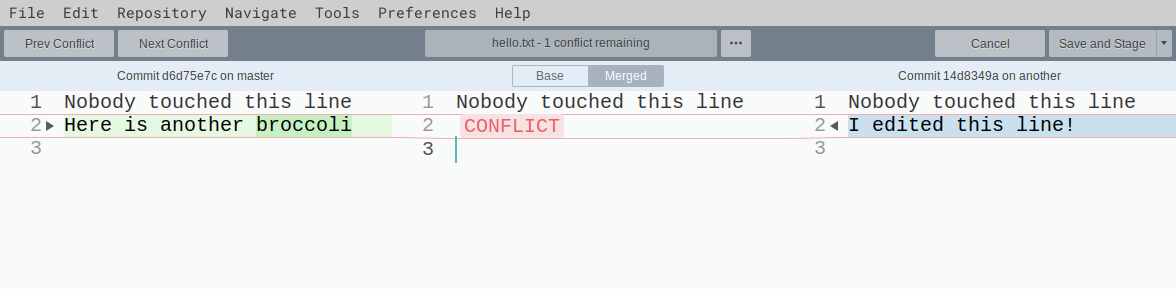
\includegraphics[width=1\textwidth]{pic/smerge}}
  \caption{Sublime Merge}
  \end{figure}
  \end{center}

  \pause
  \begin{center}
  \Large
  \texttt{pull} ist ein Alias f\"ur \texttt{fetch} + \texttt{merge}
  \end{center}
\end{frame}

\subsection{Branch}
\begin{frame}[c]{Branch}
  \begin{center}
  \scalebox{-1}[-1]{
\includegraphics[width=\textwidth]{pic/treebranch}}
  \end{center}
\end{frame}

\begin{frame}{Begriff: Branch}
\begin{center}
\resizebox{\textwidth}{!}{
\begin{tikzpicture}
  \node (loc) at (0, 0) {}
          (.5,0) node[above=.2cm] {Local};

  \begin{pgfonlayer}{bg}
  \draw[blue, fill=blue!10] ($(loc)+(-.5,1)$) rectangle ($(loc)+(6.5,-2)$);
  \end{pgfonlayer}

  \foreach \x in {0,...,1}
  {
    \draw[thick, black, fill=orange] ($(loc)+(\x, -1)$) circle [radius=.1] node[] (C\x) {};
  }

  \foreach \x in {2,...,5}
  {
    \draw[thick, black, fill=magenta] ($(loc)+(\x, -1)$) circle [radius=.1] node (CL\x) {};
    \draw[thick, black, fill=green!60!black] ($(loc)+(\x, 0)$) circle [radius=.1] node (CR\x) {};
  }

  \draw[thick, black]
    (C0) to (C1)
    (C1) to[in=200, out=30] (CR2) node [above=.5cm, right=.1] {\tiny\texttt{testing}}
    (CR2) to (CR3) to (CR4) to (CR5)
    (C1) to (CL2) node[above=.4cm, right=.1] {\tiny\texttt{master}}
    (CL2) to (CL3) to (CL4) to (CL5)
  ;

  \pause
  \draw[thick, black]
    (CR4) to[in=160, out=-20] (CL5)
  ;
\end{tikzpicture}
}
\end{center}
\end{frame}

\section{Git benutzen}

\end{document}
